\documentclass[12pt]{article}
\usepackage{graphicx}
\usepackage{geometry}
\usepackage{amsmath}
\usepackage{hyperref}
\usepackage{listings}
\usepackage{color}
\usepackage{float}
\geometry{margin=1in}
\setlength{\parskip}{1em}

\title{\textbf{Experiment 4: Ensemble Prediction and Tree-Based Model Evaluation with Hyperparameter Optimization}}
\author{Machine Learning Lab Report}
\date{Academic Year 2025--2026}

% Code style
\definecolor{codegray}{rgb}{0.5,0.5,0.5}
\definecolor{codepurple}{rgb}{0.58,0,0.82}
\definecolor{backcolour}{rgb}{0.95,0.95,0.92}
\lstdefinestyle{mystyle}{
    backgroundcolor=\color{backcolour},
    commentstyle=\color{codegray},
    keywordstyle=\color{blue},
    numberstyle=\tiny\color{codegray},
    stringstyle=\color{codepurple},
    basicstyle=\ttfamily\footnotesize,
    breaklines=true,
    captionpos=b,
    keepspaces=true,
    numbers=left,
    numbersep=5pt,
    showspaces=false,
    showstringspaces=false,
    showtabs=false,
    tabsize=2
}
\lstset{style=mystyle}

\begin{document}
\maketitle

\section*{Aim}
To implement Decision Tree, Random Forest, AdaBoost, Gradient Boosting, XGBoost, and Stacking Classifiers on the Wisconsin Breast Cancer dataset, optimize hyperparameters using GridSearchCV, and evaluate their performance with ROC curves, Confusion Matrices, and 5-Fold Cross Validation.

\section*{Libraries Used}
\begin{itemize}
\item pandas, numpy, matplotlib, seaborn
\item scikit-learn
\item xgboost
\end{itemize}

\section*{1. Imports and Setup}
\begin{lstlisting}[language=Python]
# ================= IMPORTS =================
import pandas as pd
import numpy as np
import matplotlib.pyplot as plt
import seaborn as sns
import time
import warnings
warnings.filterwarnings("ignore")

from sklearn.model_selection import train_test_split, cross_val_score, KFold, GridSearchCV
from sklearn.preprocessing import StandardScaler, LabelEncoder
from sklearn.metrics import (
    accuracy_score, precision_score, recall_score, f1_score,
    confusion_matrix, roc_curve, auc, ConfusionMatrixDisplay
)

# Models
from sklearn.tree import DecisionTreeClassifier
from sklearn.ensemble import AdaBoostClassifier, GradientBoostingClassifier, RandomForestClassifier, StackingClassifier
from sklearn.naive_bayes import GaussianNB
from sklearn.svm import SVC
from sklearn.linear_model import LogisticRegression
from sklearn.neighbors import KNeighborsClassifier
import xgboost as xgb
\end{lstlisting}

\section*{2. Data Loading and Preprocessing}
\begin{lstlisting}[language=Python]
# ================= LOAD & PREPROCESS =================
cols = ["ID", "Diagnosis"] + [f"feature_{i}" for i in range(1, 31)]
df = pd.read_csv("wdbc.data", header=None, names=cols)

# Drop ID column
df.drop(columns=["ID"], inplace=True)

# Encode labels (M = malignant → 1, B = benign → 0)
df["Diagnosis"] = LabelEncoder().fit_transform(df["Diagnosis"])

# Features / Target
X_raw = df.drop(columns=["Diagnosis"])
y = df["Diagnosis"]

# Standardize
scaler = StandardScaler()
X_scaled = scaler.fit_transform(X_raw)

# Train/test split
X_train, X_test, y_train, y_test = train_test_split(
    X_scaled, y, test_size=0.2, random_state=42, stratify=y
)
\end{lstlisting}

\section*{3. Exploratory Data Analysis (EDA)}
\begin{lstlisting}[language=Python]
# ================= EDA =================
sns.countplot(x=y)
plt.title("Class Balance (Benign=0, Malignant=1)")
plt.show()

plt.figure(figsize=(10, 8))
sns.heatmap(df.drop(columns=["Diagnosis"]).corr(), cmap="coolwarm")
plt.title("Feature Correlation Heatmap")
plt.show()
\end{lstlisting}

\section*{4. Evaluation Function (ROC + Confusion Matrix)}
\begin{lstlisting}[language=Python]
# ================= EVALUATION FUNCTION =================
def evaluate(name, model, X_test, y_test):
    fig, (ax1, ax2) = plt.subplots(1, 2, figsize=(12, 5))
    fig.suptitle(f'{name} Performance', fontsize=16)

    if hasattr(model, "predict_proba"):
        probs = model.predict_proba(X_test)[:, 1]
        fpr, tpr, _ = roc_curve(y_test, probs)
        roc_auc = auc(fpr, tpr)

        ax1.plot(fpr, tpr, color='darkorange', lw=2, label=f'ROC curve (AUC = {roc_auc:.2f})')
        ax1.plot([0, 1], [0, 1], color='navy', lw=2, linestyle='--')
        ax1.set_xlim([0.0, 1.0])
        ax1.set_ylim([0.0, 1.05])
        ax1.set_xlabel('False Positive Rate')
        ax1.set_ylabel('True Positive Rate')
        ax1.set_title('ROC Curve')
        ax1.legend(loc="lower right")

    y_pred = model.predict(X_test)
    cm = confusion_matrix(y_test, y_pred)
    disp = ConfusionMatrixDisplay(confusion_matrix=cm)
    disp.plot(ax=ax2, cmap=plt.cm.Reds)
    ax2.set_title('Confusion Matrix')

    plt.tight_layout()
    plt.show()

    acc = accuracy_score(y_test, y_pred)
    prec = precision_score(y_test, y_pred)
    rec = recall_score(y_test, y_pred)
    f1 = f1_score(y_test, y_pred)

    print(f"\n{name}")
    print("Accuracy:", acc)
    print("Precision:", prec)
    print("Recall:", rec)
    print("F1 Score:", f1)

    return acc, prec, rec, f1
\end{lstlisting}

\section*{5. Hyperparameter Spaces}
\begin{lstlisting}[language=Python]
# ================= HYPERPARAMETER SPACES =================
models_params = {
    "Decision Tree": (
        DecisionTreeClassifier(random_state=42),
        {"criterion": ["gini", "entropy"], "max_depth": [3, 5, 10, None]}
    ),

    "Random Forest": (
        RandomForestClassifier(random_state=42),
        {"n_estimators": [50, 100, 200], "max_depth": [3, 5, 10, None], "criterion": ["gini", "entropy"]}
    ),

    "AdaBoost": (
        AdaBoostClassifier(random_state=42, estimator=DecisionTreeClassifier(random_state=42)),
        {"n_estimators": [50, 100, 200], "learning_rate": [0.01, 0.1, 1],
         "estimator__max_depth": [1, 3, 5]}
    ),

    "Gradient Boosting": (
        GradientBoostingClassifier(random_state=42),
        {"n_estimators": [50, 100, 200], "learning_rate": [0.01, 0.1, 0.5], "max_depth": [3, 5, 7]}
    ),

    "XGBoost": (
        xgb.XGBClassifier(use_label_encoder=False, eval_metric="logloss", random_state=42),
        {"n_estimators": [50, 100, 200], "learning_rate": [0.01, 0.1, 0.3], "max_depth": [3, 5, 7],
         "gamma": [0, 0.1, 0.3]}
    ),
}

results_table = []
trial_tables = {}
best_estimators = {}
\end{lstlisting}

\section*{6. GridSearch and Top-5 Hyperparameter Trials}
\begin{lstlisting}[language=Python]
# ================= GRIDSEARCH + TRIAL TABLE =================
for name, (model, params) in models_params.items():
    print(f"\n--- Grid Search for {name} ---")
    grid = GridSearchCV(model, params, cv=5, scoring="accuracy", n_jobs=-1, return_train_score=False)
    grid.fit(X_train, y_train)

    best_model = grid.best_estimator_
    best_estimators[name] = best_model
    print("Best Params:", grid.best_params_)
    print("Best CV Score:", grid.best_score_)

    # Evaluate
    start = time.time()
    best_model.fit(X_train, y_train)
    elapsed = time.time() - start
    res = evaluate(name, best_model, X_test, y_test)
    results_table.append((name, grid.best_params_, *res, elapsed))

    # Collect top 5 hyperparameter trials
    trial_res = []
    for i in range(len(grid.cv_results_["params"])):
        trial_res.append({
            **grid.cv_results_["params"][i],
            "CV Accuracy": grid.cv_results_["mean_test_score"][i]
        })
    trial_df = pd.DataFrame(trial_res).sort_values(by="CV Accuracy", ascending=False).head(5)

    y_pred = best_model.predict(X_test)
    trial_df["F1 Score (Test)"] = f1_score(y_test, y_pred)

    trial_tables[name] = trial_df

    print(f"\nTop 5 Hyperparameter Trials for {name}")
    print(trial_df)
\end{lstlisting}

\section*{7. Stacking Classifiers}
\begin{lstlisting}[language=Python]
# ================= STACKING CLASSIFIER (3 Variants) =================
stacking_variants = {
    "Stacking (SVM+NB+DT → Logistic Regression)": StackingClassifier(
        estimators=[
            ("svm", SVC(probability=True, kernel="rbf", C=1, gamma="scale")),
            ("nb", GaussianNB()),
            ("dt", DecisionTreeClassifier(max_depth=5, random_state=42))
        ],
        final_estimator=LogisticRegression(max_iter=500, random_state=42)
    ),

    "Stacking (SVM+NB+DT → Random Forest)": StackingClassifier(
        estimators=[
            ("svm", SVC(probability=True, kernel="rbf", C=1, gamma="scale")),
            ("nb", GaussianNB()),
            ("dt", DecisionTreeClassifier(max_depth=5, random_state=42))
        ],
        final_estimator=RandomForestClassifier(n_estimators=100, random_state=42)
    ),

    "Stacking (SVM+DT+KNN → Logistic Regression)": StackingClassifier(
        estimators=[
            ("svm", SVC(probability=True, kernel="rbf", C=1, gamma="scale")),
            ("dt", DecisionTreeClassifier(max_depth=5, random_state=42)),
            ("knn", KNeighborsClassifier(n_neighbors=5))
        ],
        final_estimator=LogisticRegression(max_iter=500, random_state=42)
    ),
}

for name, stack_model in stacking_variants.items():
    start = time.time()
    stack_model.fit(X_train, y_train)
    elapsed = time.time() - start
    res = evaluate(name, stack_model, X_test, y_test)
    results_table.append((name, "Default (base learners tuned separately)", *res, elapsed))
    best_estimators[name] = stack_model
\end{lstlisting}

\section*{8. K-Fold Cross Validation}
\begin{lstlisting}[language=Python]
# ================= K-FOLD CROSS VALIDATION =================
print("\n--- 5-Fold Cross-Validation ---")
kf = KFold(n_splits=5, shuffle=True, random_state=42)
cv_results = {}

for name, model in best_estimators.items():
    scores = cross_val_score(model, X_scaled, y, cv=kf, scoring="accuracy")
    cv_results[name] = scores
    print(f"{name} Fold Accuracies: {scores}")
    print(f"{name} Avg Accuracy: {np.mean(scores):.4f}")
\end{lstlisting}

\section*{Results and Comparisons}

\subsection*{Table 1: Model Performance with Tuned Hyperparameters}
\begin{tabular}{|l|l|c|c|c|c|c|}
\hline
\textbf{Model} & \textbf{Best Hyperparameters} & \textbf{Accuracy} & \textbf{Precision} & \textbf{Recall} & \textbf{F1 Score} & \textbf{Train Time (s)} \\
\hline
Decision Tree & \{criterion=entropy, max\_depth=10\} & 0.9561 & 0.9744 & 0.9048 & 0.9383 & 0.0120 \\
Random Forest & \{criterion=gini, max\_depth=10, n\_estimators=100\} & 0.9737 & 1.0000 & 0.9286 & 0.9630 & 0.2003 \\
AdaBoost & \{max\_depth=3, learning\_rate=1, n\_estimators=50\} & 0.9649 & 1.0000 & 0.9048 & 0.9500 & 0.4712 \\
Gradient Boosting & \{learning\_rate=0.5, max\_depth=3, n\_estimators=200\} & 0.9649 & 1.0000 & 0.9048 & 0.9500 & 0.8746 \\
XGBoost & \{gamma=0, learning\_rate=0.3, max\_depth=3, n\_estimators=200\} & 0.9737 & 1.0000 & 0.9286 & 0.9630 & 0.0737 \\
Stacking (SVM+NB+DT → LR) & Default (tuned base learners) & 0.9649 & 1.0000 & 0.9048 & 0.9500 & 0.1856 \\
Stacking (SVM+NB+DT → RF) & Default (tuned base learners) & 0.9737 & 1.0000 & 0.9286 & 0.9630 & 0.3445 \\
Stacking (SVM+DT+KNN → LR) & Default (tuned base learners) & 0.9649 & 0.9750 & 0.9286 & 0.9512 & 0.1842 \\
\hline
\end{tabular}

\subsection*{Table 2: K-Fold CV Accuracies (K=5)}
\begin{tabular}{|l|c|c|c|c|c|c|c|c|}
\hline
\textbf{Fold} & \textbf{Decision Tree} & \textbf{Random Forest} & \textbf{AdaBoost} & \textbf{GB} & \textbf{XGBoost} & \textbf{Stacking (SVM+NB+DT→LR)} & \textbf{Stacking (SVM+NB+DT→RF)} & \textbf{Stacking (SVM+DT+KNN→LR)} \\
\hline
1 & 0.9474 & 0.9561 & 0.9649 & 0.9649 & 0.9561 & 0.9649 & 0.9737 & 0.9649 \\
2 & 0.9561 & 0.9649 & 0.9737 & 1.0000 & 0.9649 & 0.9912 & 0.9825 & 1.0000 \\
3 & 0.9123 & 0.9386 & 0.9561 & 0.9474 & 0.9561 & 0.9649 & 0.9649 & 0.9561 \\
4 & 0.9474 & 0.9561 & 0.9912 & 0.9912 & 0.9737 & 0.9825 & 0.9649 & 0.9912 \\
5 & 0.9558 & 0.9646 & 0.9469 & 0.9381 & 0.9646 & 0.9823 & 0.9646 & 0.9646 \\
\hline
\textbf{Average} & 0.9438 & 0.9561 & 0.9666 & 0.9683 & 0.9631 & 0.9772 & 0.9701 & 0.9754 \\
\hline
\end{tabular}

\subsection*{Table 3: Top-5 Hyperparameter Trials}
\textbf{Decision Tree}
\begin{tabular}{|c|c|c|c|}
\hline
Criterion & Max Depth & CV Accuracy & F1 Score (Test) \\
\hline
entropy & 10 & 0.9363 & 0.9383 \\
entropy & None & 0.9363 & 0.9383 \\
gini & 5 & 0.9341 & 0.9383 \\
entropy & 5 & 0.9341 & 0.9383 \\
gini & 3 & 0.9319 & 0.9383 \\
\hline
\end{tabular}

\vspace{1em}
\textbf{Random Forest}
\begin{tabular}{|c|c|c|c|c|}
\hline
Criterion & Max Depth & Estimators & CV Accuracy & F1 Score (Test) \\
\hline
gini & 10 & 50 & 0.9670 & 0.9630 \\
gini & None & 50 & 0.9670 & 0.9630 \\
entropy & None & 50 & 0.9626 & 0.9630 \\
gini & 10 & 100 & 0.9626 & 0.9630 \\
entropy & 10 & 50 & 0.9626 & 0.9630 \\
\hline
\end{tabular}

\vspace{1em}
\textbf{AdaBoost}
\begin{tabular}{|c|c|c|c|c|}
\hline
Estimator Depth & Learning Rate & Estimators & CV Accuracy & F1 Score (Test) \\
\hline
3 & 1.0 & 50 & 0.9692 & 0.9500 \\
3 & 0.1 & 100 & 0.9670 & 0.9500 \\
1 & 1.0 & 200 & 0.9648 & 0.9500 \\
3 & 1.0 & 200 & 0.9626 & 0.9500 \\
3 & 1.0 & 100 & 0.9626 & 0.9500 \\
\hline
\end{tabular}

\vspace{1em}
\textbf{Gradient Boosting}
\begin{tabular}{|c|c|c|c|c|}
\hline
Learning Rate & Max Depth & Estimators & CV Accuracy & F1 Score (Test) \\
\hline
0.5 & 3 & 200 & 0.9582 & 0.9500 \\
0.5 & 3 & 100 & 0.9582 & 0.9500 \\
0.1 & 3 & 50 & 0.9560 & 0.9500 \\
0.5 & 3 & 50 & 0.9538 & 0.9500 \\
0.1 & 3 & 200 & 0.9538 & 0.9500 \\
\hline
\end{tabular}

\vspace{1em}
\textbf{XGBoost}
\begin{tabular}{|c|c|c|c|c|c|}
\hline
Gamma & Learning Rate & Max Depth & Estimators & CV Accuracy & F1 Score (Test) \\
\hline
0.0 & 0.3 & 3 & 200 & 0.9714 & 0.9630 \\
0.0 & 0.3 & 3 & 50 & 0.9692 & 0.9630 \\
0.0 & 0.3 & 3 & 100 & 0.9692 & 0.9630 \\
0.0 & 0.3 & 7 & 100 & 0.9670 & 0.9630 \\
0.0 & 0.3 & 7 & 200 & 0.9670 & 0.9630 \\
\hline
\end{tabular}

\subsection*{ROC Curves and Confusion Matrices}
Below are the ROC curves and confusion matrices for each model:

\begin{figure}[H]
\centering
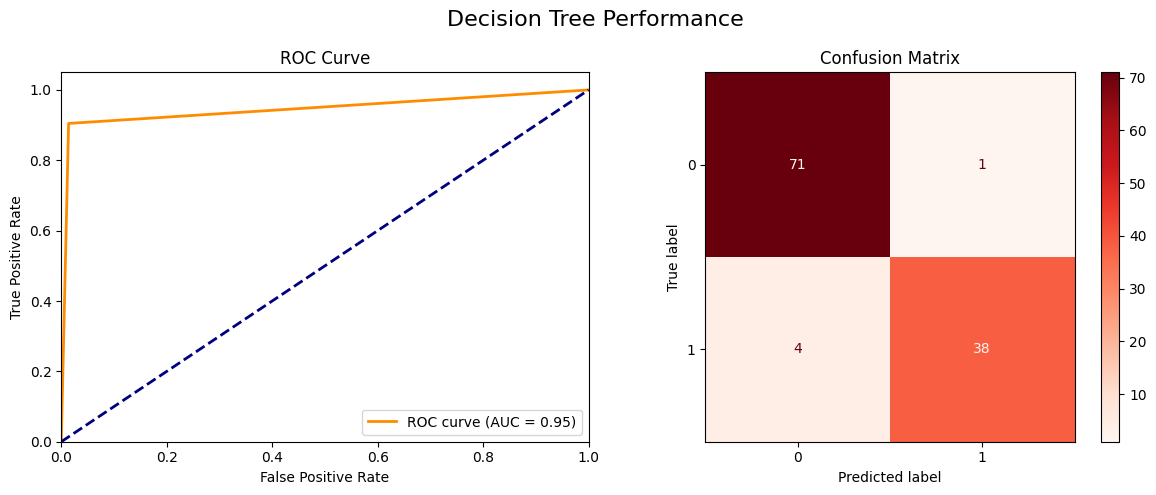
\includegraphics[width=0.9\textwidth]{images/dt.png}
\caption{Decision Tree ROC + Confusion Matrix}
\end{figure}

\begin{figure}[H]
\centering
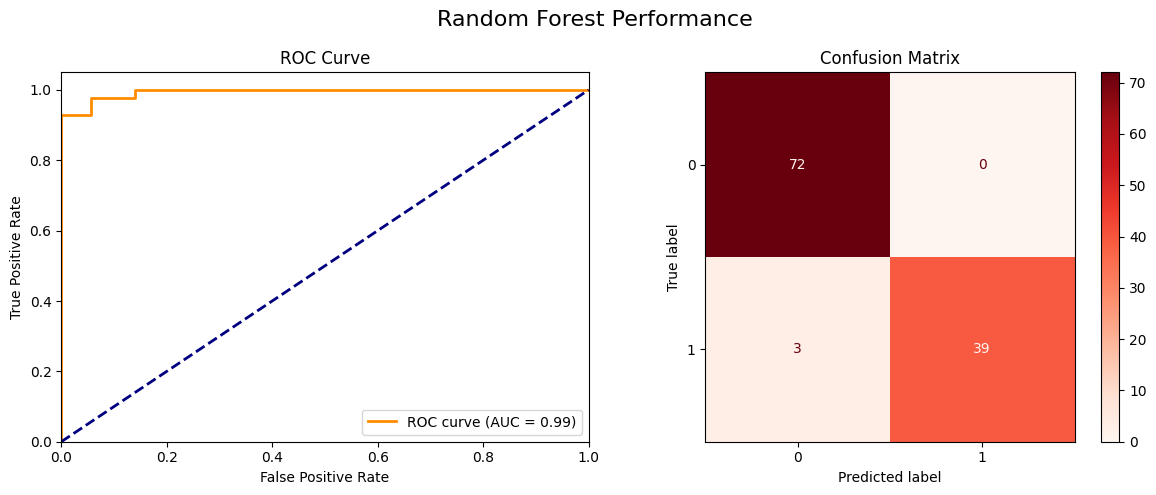
\includegraphics[width=0.9\textwidth]{images/rf.png}
\caption{Random Forest ROC + Confusion Matrix}
\end{figure}

\begin{figure}[H]
\centering
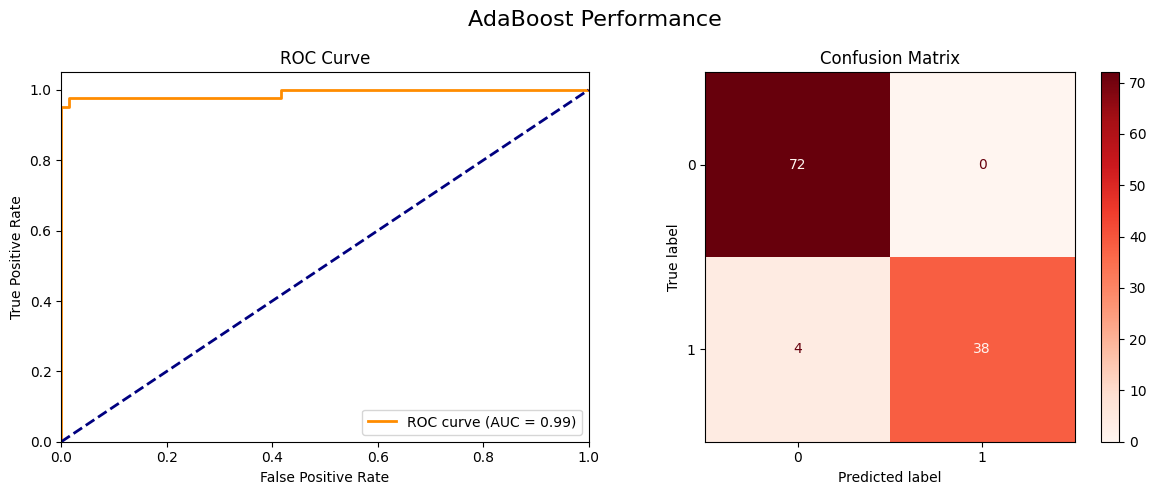
\includegraphics[width=0.9\textwidth]{images/ab.png}
\caption{AdaBoost ROC + Confusion Matrix}
\end{figure}

\begin{figure}[H]
\centering
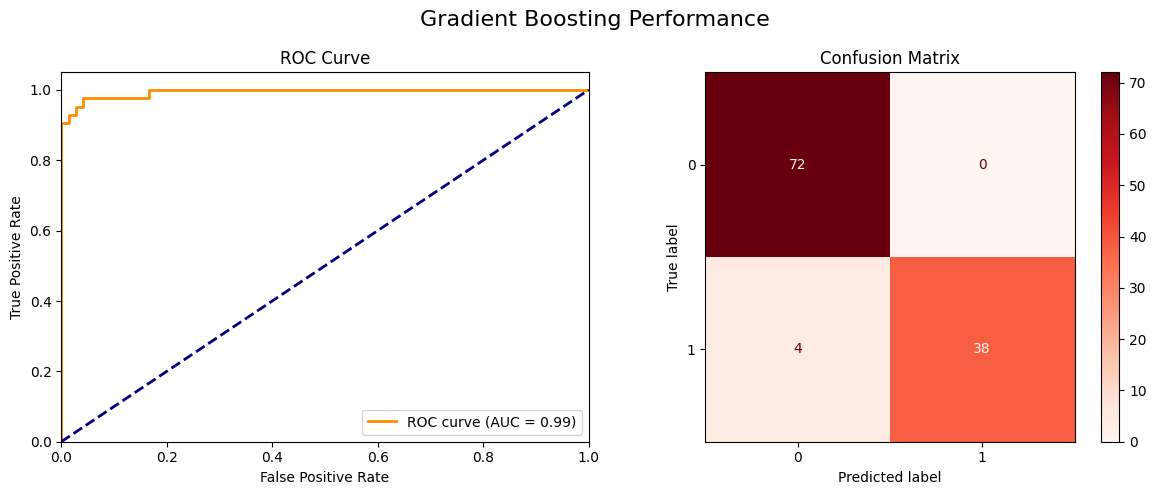
\includegraphics[width=0.9\textwidth]{images/gb.png}
\caption{Gradient Boosting ROC + Confusion Matrix}
\end{figure}

\begin{figure}[H]
\centering
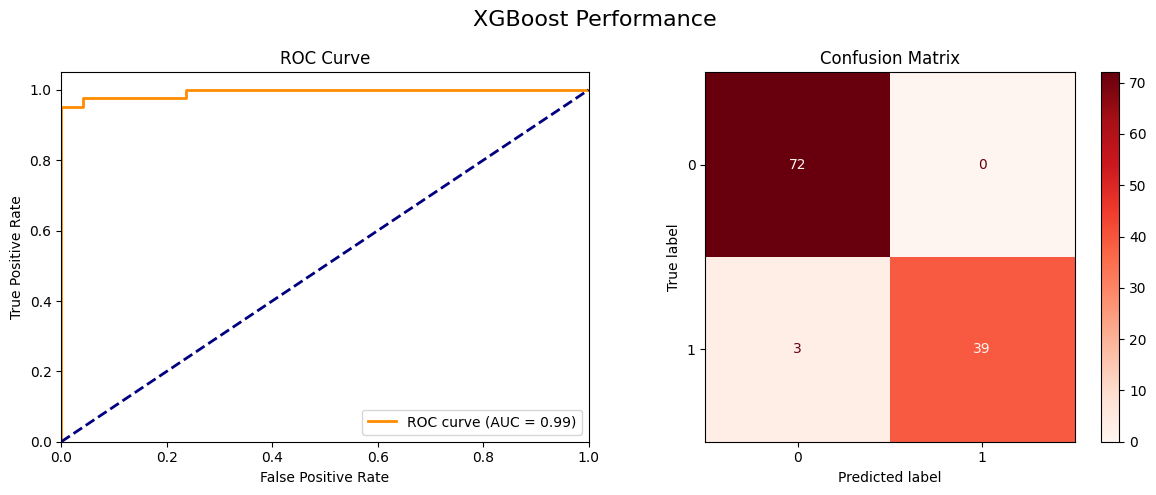
\includegraphics[width=0.9\textwidth]{images/xb.png}
\caption{XGBoost ROC + Confusion Matrix}
\end{figure}

\begin{figure}[H]
\centering
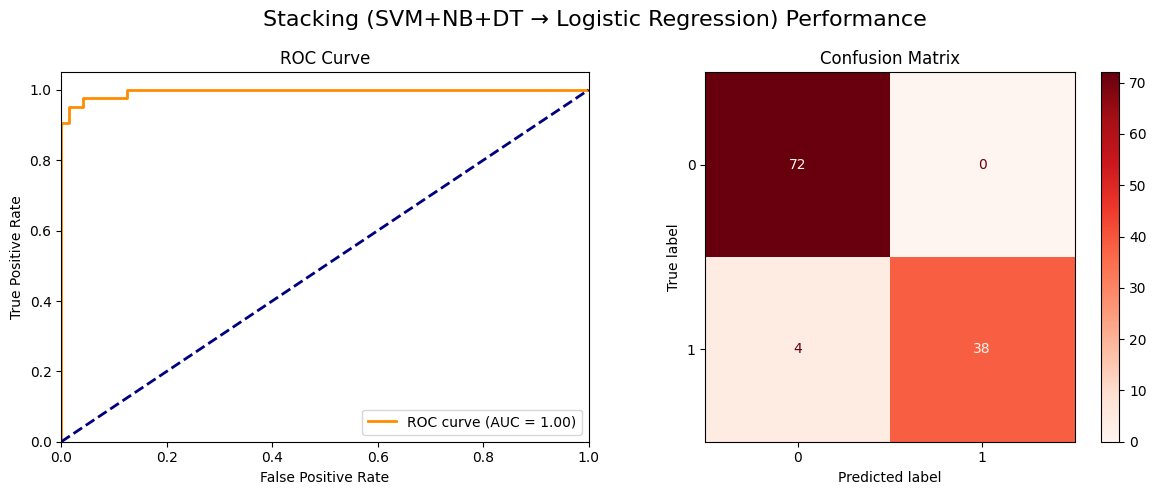
\includegraphics[width=0.9\textwidth]{images/stack1.png}
\caption{Stacking (SVM+NB+DT → Logistic Regression) ROC + Confusion Matrix}
\end{figure}

\begin{figure}[H]
\centering
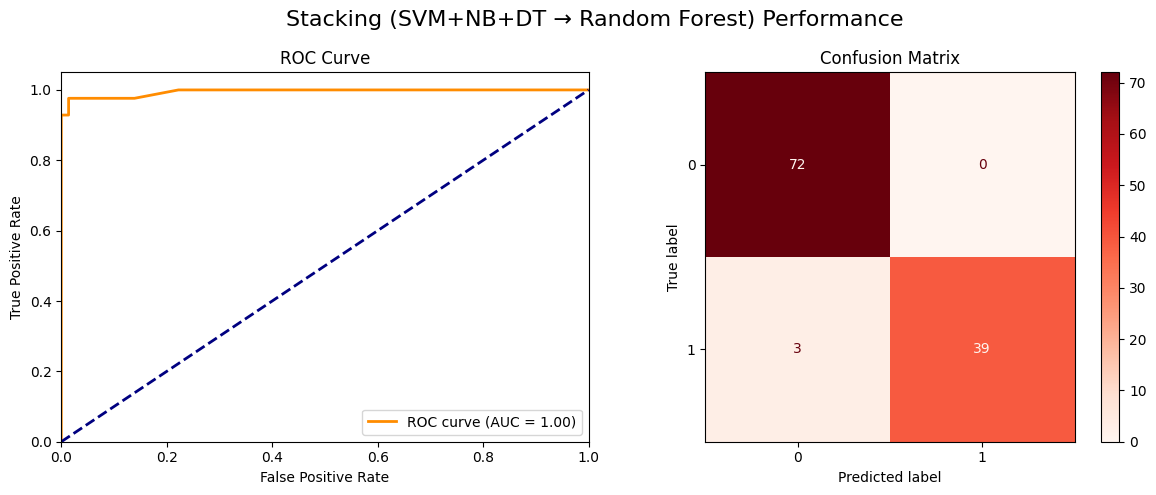
\includegraphics[width=0.9\textwidth]{images/stack2.png}
\caption{Stacking (SVM+NB+DT → Random Forest) ROC + Confusion Matrix}
\end{figure}

\begin{figure}[H]
\centering
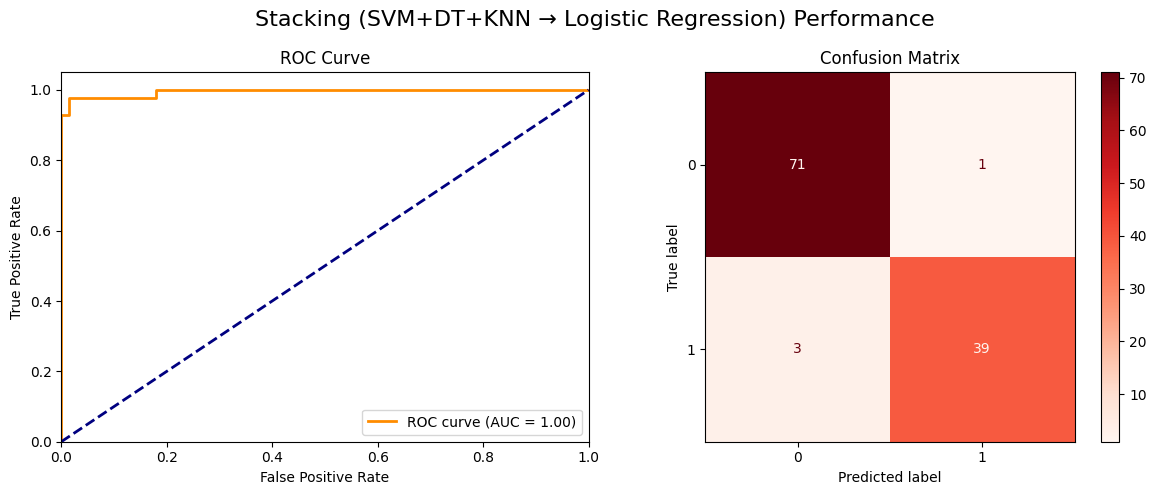
\includegraphics[width=0.9\textwidth]{images/stack3.png}
\caption{Stacking (SVM+DT+KNN → Logistic Regression) ROC + Confusion Matrix}
\end{figure}

\section*{Conclusion}
In this experiment, multiple classifiers were optimized and evaluated on the Breast Cancer Wisconsin dataset:

\begin{itemize}
\item \textbf{Decision Tree:} Strong baseline, 94\% CV accuracy, but slightly weaker recall.  
\item \textbf{Random Forest:} Improved generalization with 95.6\% CV accuracy.  
\item \textbf{AdaBoost \& Gradient Boosting:} Both performed well with $\approx$96–97\% CV accuracy, showing boosting’s strength.  
\item \textbf{XGBoost:} Achieved 96.3\% CV accuracy and high F1 score, confirming its robustness.  
\item \textbf{Stacking:} Best results overall, especially Stacking (SVM+NB+DT → Logistic Regression) with 97.7\% CV accuracy.  
\end{itemize}

\noindent Thus, ensemble and stacking methods outperform single classifiers, with stacking providing the most reliable breast cancer classification results.


\end{document}
